
In this section we provide an analysis of the classes of errors observed in
production-grade software-defined networks. We base our analysis on conversations with
researchers at Nicira~\cite{nicira}, a startup focused on developing a network operating
system for production SDN deployments~\cite{onix}.

\begin{figure}[t]
    \centering
    \begin{tabular}{ccc}
    \hspace{-3pt}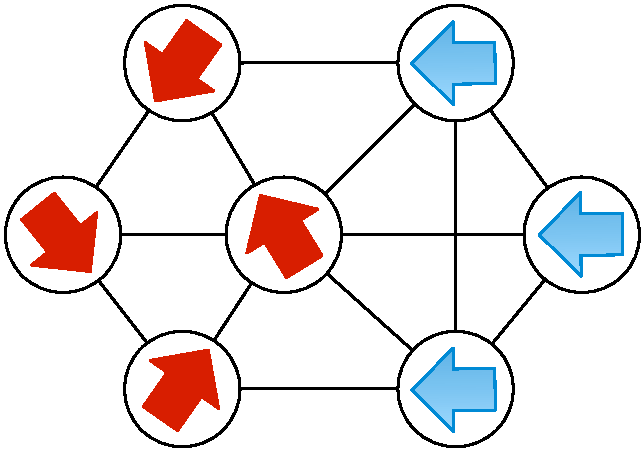
\includegraphics[width=1in]{../diagrams/bugs/loop.pdf}&
    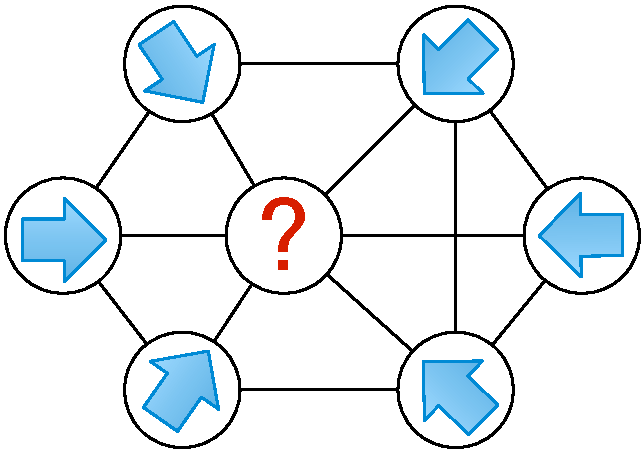
\includegraphics[width=1in]{../diagrams/bugs/dead_end.pdf}&
    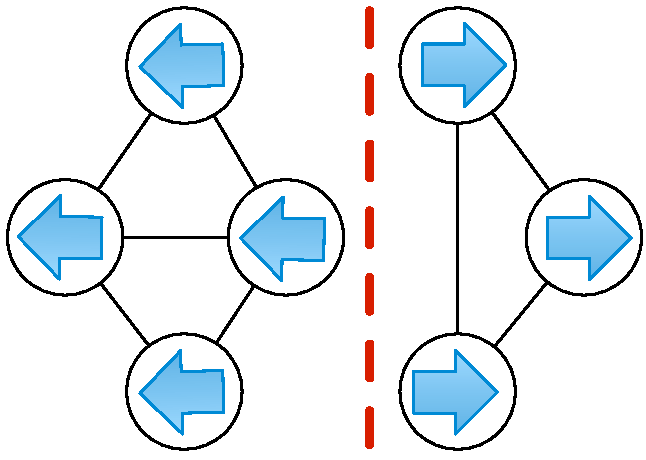
\includegraphics[width=1in]{../diagrams/bugs/partition.pdf}\\
    {\bf (i) Loop}&{\bf (ii) Black Hole}&{\bf (iii) Partition}\\
    \end{tabular}
    \caption[]{\label{fig:invariantviolations} Selected classes of physical network errors detectable with static
    checking.\vspace{-10pt}} 
\end{figure}

\colin{Insert diagrams on bugs that we can catch but Anteater can't}

What kind of bugs do we want to analyze? Well I guess we start with static
bugs that Anteater can detect. Useful for providing background common error
conditions seen in networks. 

Well, loops are these things where packets go in a circle and never come out.
Their bad because they cause the traffic stuck in the loop to never go
through. They're also bad because they congest the routers in the loop, and
therefore affect unrelated traffic. Really bad at layer 2, where there are no
ttls.

Ok. Then there are partitions. In most cases, every host in the network should
be able to reach every other host in the network. If there exists no route to
one host, 

Blackholes are a related problem. Traffic may arrive at a dead end,

Maybe talk about routing consistency? Simplest invariant is `No packet can
arrive at a web server without passing through a firewall`. If re-distributing
load across ingress switches, in-flight packets might get the web server
without passing through a firewall.

Ok, now for the interesting bugs. Start with Justine's flow overlap bug.

Then go on to virtualization bugs. These are pretty severe, by the way.
Semantic mismatches, yahdah yahdah.

Then consistency. 9 in 10 systems researchers agree, PAXOS is hard.

